
\documentclass[9pt,landscape]{extarticle}
\usepackage{amssymb,amsmath,amsthm,amsfonts}
\usepackage{multicol,multirow}
\usepackage{calc}
\usepackage{ifthen}
\usepackage[landscape]{geometry}
\usepackage[colorlinks=true,citecolor=blue,linkcolor=blue]{hyperref}
\usepackage{graphicx}
\usepackage{commath}
\usepackage{listings}
\usepackage{microtype}
\usepackage[compact,small]{titlesec}
\usepackage{enumitem}
\setenumerate{noitemsep,topsep=0pt,parsep=0pt,partopsep=0pt}
\setitemize{noitemsep,topsep=0pt,parsep=0pt,partopsep=0pt}
\graphicspath{ {./images/} }
\ifthenelse{\lengthtest { \paperwidth = 11in}}
    { \geometry{top=.5cm,left=.5cm,right=.5cm,bottom=.5cm} }
	{\ifthenelse{ \lengthtest{ \paperwidth = 297mm}}
		{\geometry{top=1cm,left=1cm,right=1cm,bottom=1cm} }
		{\geometry{top=1cm,left=1cm,right=1cm,bottom=1cm} }
	}
\pagestyle{empty}
\makeatletter
\renewcommand{\section}{\@startsection{section}{1}{0mm}%
                                {-1ex plus -.5ex minus -.2ex}%
                                {0.5ex plus .2ex}%x
                                {\normalfont\large\bfseries}}
\renewcommand{\subsection}{\@startsection{subsection}{2}{0mm}%
                                {-1ex plus -.5ex minus -.2ex}%
                                {0.3ex}%
                                {\normalfont\small\bfseries}}
\makeatother
\setcounter{secnumdepth}{0}
\setlength{\parindent}{0pt}
\setlength{\parskip}{0pt plus 0.5ex}
% -----------------------------------------------------------------------

\title{Cheat sheet}

\begin{document}

\raggedright
\footnotesize

\begin{center}
     \Large{\textbf{Computational Structure - Cheatsheet - Quiz 1}} \\
\end{center}
\begin{multicols*}{6}
\setlength{\premulticols}{1pt}
\setlength{\postmulticols}{1pt}
\setlength{\multicolsep}{1pt}
\setlength{\columnsep}{2pt}

\section{Information}
information $\propto$ uncertainty $\propto$ $\frac{1}{p} $ \\
In laymen terms: If an event is bound to happen, then the fact that the event happens does not give any kind of information  \\
$I(X) $ = $\log_{2} \frac{1}{p_{i}} $ \\
$I(X)_{N \to M} $ = $\log_{2} \frac{N}{M} $ bits , where N is the number of equally probably choice with M possible choices\\

\section{2's complement}
Step 1 : Inverse \\
Step 2 : Add 1 to binary \\ 
\smallskip
\subsection{Number Range}
Given X bits \\
$-$Signed bit : $ -2^{x-1}$ to $2^{x-1} - 1$ \\
$-$Unsigned bit : 0 to $2^{x} - 1$ \\
$-$We can encode 2X choices, or random variables
 
 \section{CMOS Recipe}
$-$Only use NFETs in pulldown circuits and PFETs in pullup circuits \\
$-$ PO-NI - PFETs conducts when 0, NFETs when 1
$-$ AB is parallel in PD, but series in PU.
$-$ Ensure no direct connection from VDD to GND
\section{Combinational Device}
\begin{enumerate}
 \item Inputs
 \item Outputs
 \item Functional specification that details the output for each input
 \item The propagation time to get a valid output given a valid input
\end{enumerate}
\subsection{Static Discipline}
Propagation time to get valid output given valid input

\section{VTC}
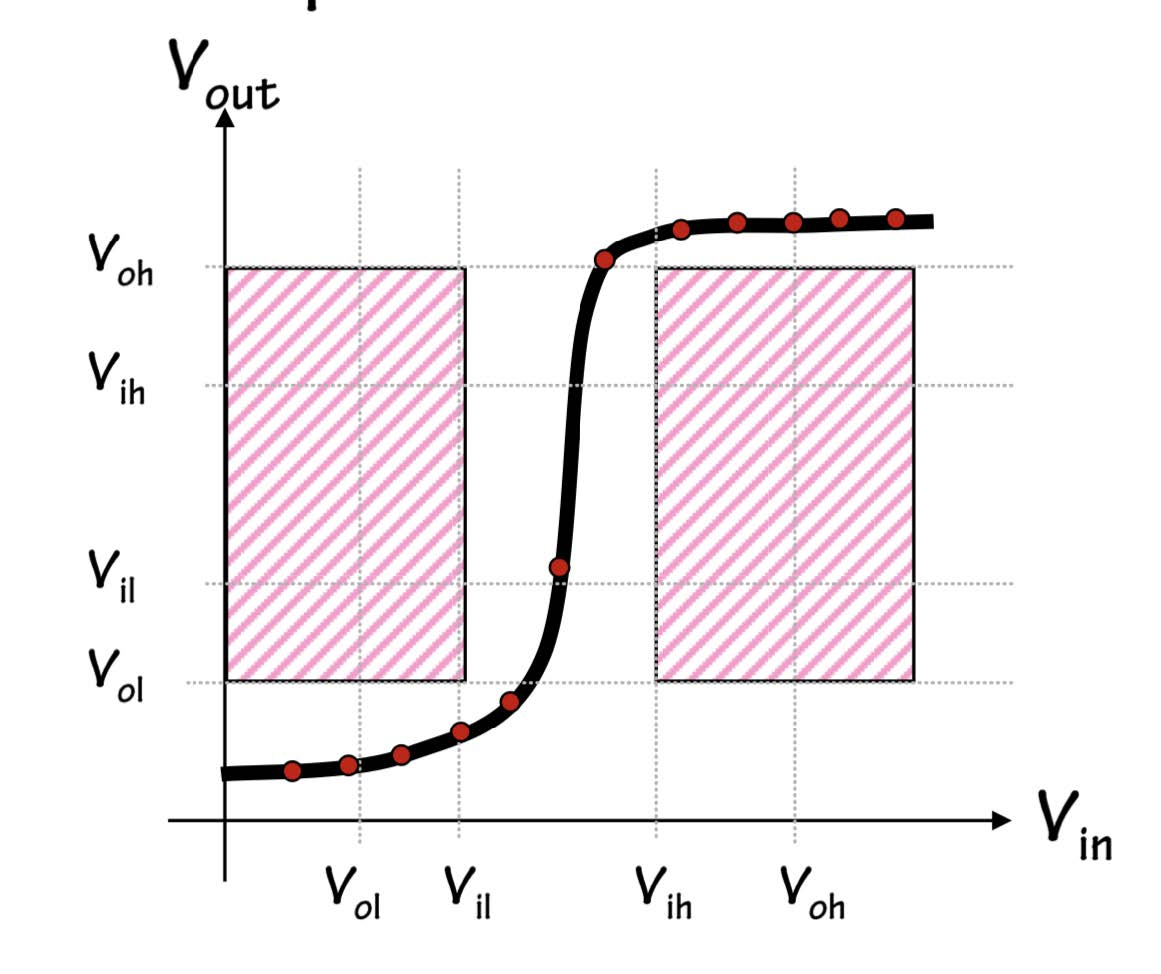
\includegraphics[width = 3.5cm]{VTC} \\
\begin{enumerate}
 \item Gain > 1
 \item Non-Linear Gain
\end{enumerate}

\section{Noise Margin}
\begin{enumerate}
 \item $V_{ol}$ or $V_{oh}$ is the voltage that your system outputs, depending on whether its ’0’ or ’1’. It is going to be received by another system after traversing through some wire.
 \item $V_{ih}$ or $V_{ih}$ is the voltage that your system receive as input from another system.
 \item Wire has noise, it can cause voltages to change as it traverse through it
\end{enumerate}


\section{The MOSFET}
\begin{enumerate}
 \item The current flow between source and drain IDS is proportional to W=L (the
width and the length) of the FET.
 \item The side with the higher potential is drain, the one with the lower potential
is source.
\item The p-type : majority care holes (impurities), bulk is connected to VDD
\item The n-type : majority are electrons, bulk is connected to GND
\item A FET that is ”ON” means that there’s connection between D and S, current
can flow through them. 
\end{enumerate}

\section{Timings}
\begin{enumerate}
 \item The Propagation Delay $t_{pd}$ - the time delay from valid input to valid output. The effective tpd of an entire
circuit is the maximum cumulative propagation delay over all paths from inputs to outputs.
\item The Contamination Delay $t_{cd}$ - the time delay from invalid input to invalid output. The effective tcd of an
entire circuit is the minimum cumulative contamination delay over all paths from
inputs to outputs.
\end{enumerate}
 
 \section{Logic Synthesis}
 \subsection{NAND and NOR gates}
 NANDs and NORs are universal, meaning that they can implement any boolean function. AND, OR, and INV aren’t sufficient. We can use NANDs and NORs to make AND, OR and INV: \\
 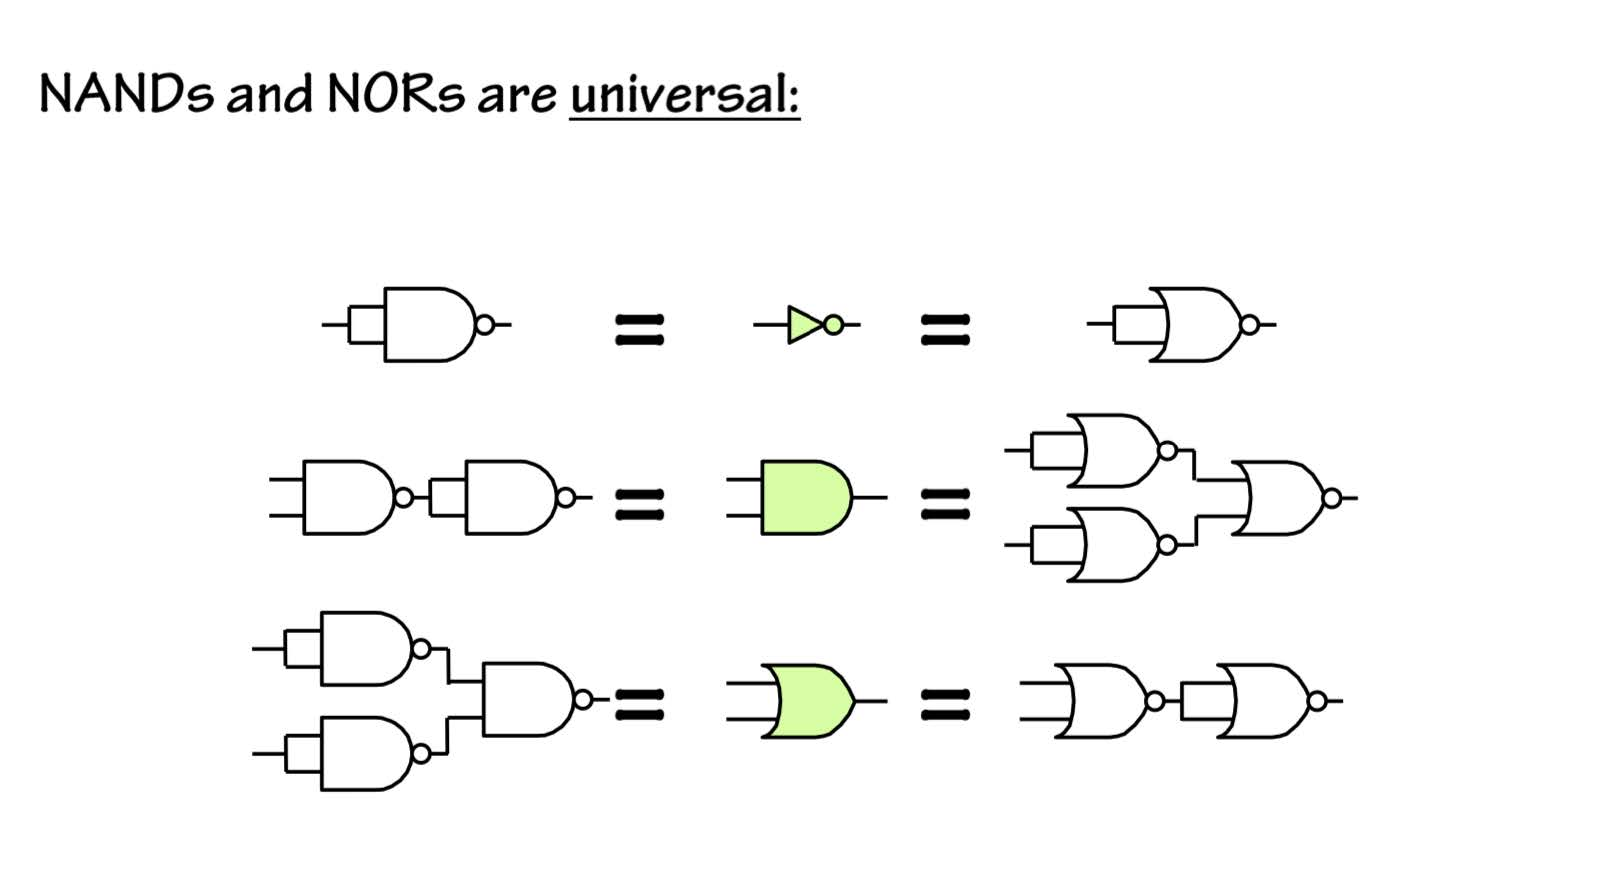
\includegraphics[width = 4.5cm]{NAND_NOR}
 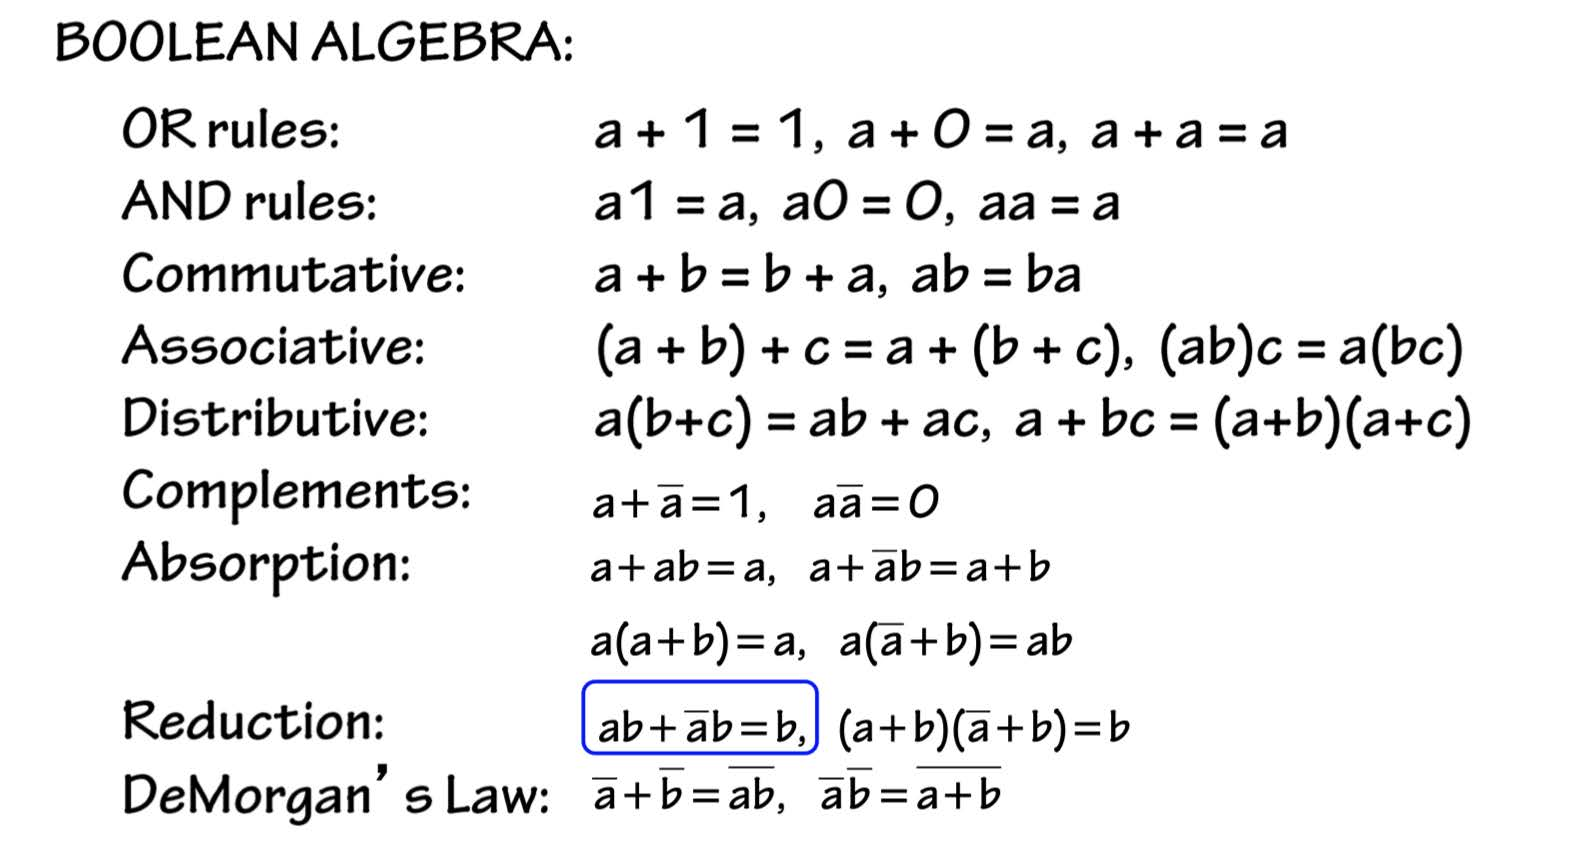
\includegraphics[width = 4.5cm]{boolean}
 \subsection{Karnaugh Map}
 \begin{enumerate}
\item ”1” cells, No diagonal grouping, Cells can overlap.
\item The top/bottom and left/right edges of map are continuous
\end{enumerate}
 
\section{Multiplexer (MUX)}
It is made up of logic gates (INV, AND, and OR, or
NANDs).\\
  \begin{enumerate}
 \item Muxes are universal,
\item A Mux can have $2^{k}$ data inputs, and k bits select inputs, and only can have 1
output
\item A mux always has three components: the inputs, the selector
signal(s), and the output. 
\end{enumerate}
 \section{Decoder}
   \begin{enumerate}
 \item A Decoder is the opposite of Mux
\item It has k select inputs, and $2^{k}$ possible data outputs
\item The selected output i is HIGH (1), and the rest of the $2^{k} - 1$ data output is LOW
(0).
\end{enumerate}
\subsection{Read-Only-Memories (ROM)}
A decoder’s function is to create a read-only-memories.
 

\begin{enumerate}
\item ROMs ignore the structure of combinational functions (hardcoded)
\item The selectors are like ”addresses” of an entry
\item For an N-input boolean function, the size of ROM is roughly $2^{N} x$  number of outputs.
For example, the Full Adder has 3 inputs (A, B, $C_{in}$), and 2 outputs (S and
$C_{out}$). Hence the size of the ROM is $2^{3} x 2 = 16$.
\end{enumerate}

\subsection{Schematic explanation} 
\begin{enumerate}
\item At the output of the decoder, the little circuit with inverted triangle symbol
signifies a pulldown circuit (connected to ground), which will ”drain” a signal
into 0.
\item At each combination of A, B, and Ci , only one of the 8 outputs of the decoder
will be 1. For example, when A = 0;B = 0;Ci = 1, the second output from the
top is 1. There’s a pulldown for S (it is connected to the ground), which makes
it 0, and no pulldown for the $C_{out}$ , which makes it 1.
\item Note the presence of inverters
\item By invention, the location of the ”pulldown” circuits correspond to a 1 in the
truth table for that particular output (S or Cout).
\end{enumerate}

\section{Week 3}
\section{D-Latch}
Mux with a feedback loop
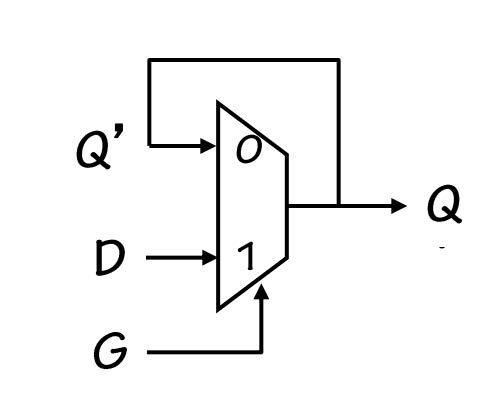
\includegraphics[width = 4.5cm]{D_latch}
-G represents the clock signal \\
-When G is 1, D is selected in the mux. (Write Mode) \\
-When G is 0,  Q follows Q'. (Read memory mode) \\
\section{The Dynamic Discipline}
The input to a synchronous sequential circuit must be stable
during the aperture (setup and hold) time around the clock
edge.
The dynamic discipline states that
\begin{enumerate}
\item $T_{setup} = 2t_{pd}$
\item $T_{hold} = t_{pd}$
\end{enumerate}
\begin{enumerate}
\item $T_{setup}$ = the minimum amount of time that the voltage on wire D needs to be stable before the clock edge changes from 0 to 1.
\item $T_{hold}$ = the minimum amount of time that the voltage on wire D needs to be stable after the clock edge changes from 0 to 1.
\item $t_{pd}$ is the propagation delay of the D-latch
\end{enumerate}
\section{Flip-Flop}
Created by putting 2 D-latches in series \\

\begin{enumerate}
\item There is an inverter on the G input on the master flip flop
\item When CLK signal is 0, the G wire of master latch receive a 1 while slave flip flop receive a 0 \\
Master latch : Write mode \\
Slave latch : Read mode
\item Vice-versa when CLk signal is 1
\item 1 D-Latch is on write mode why 1 D-latch is on memory mode at anytime.
\end{enumerate}
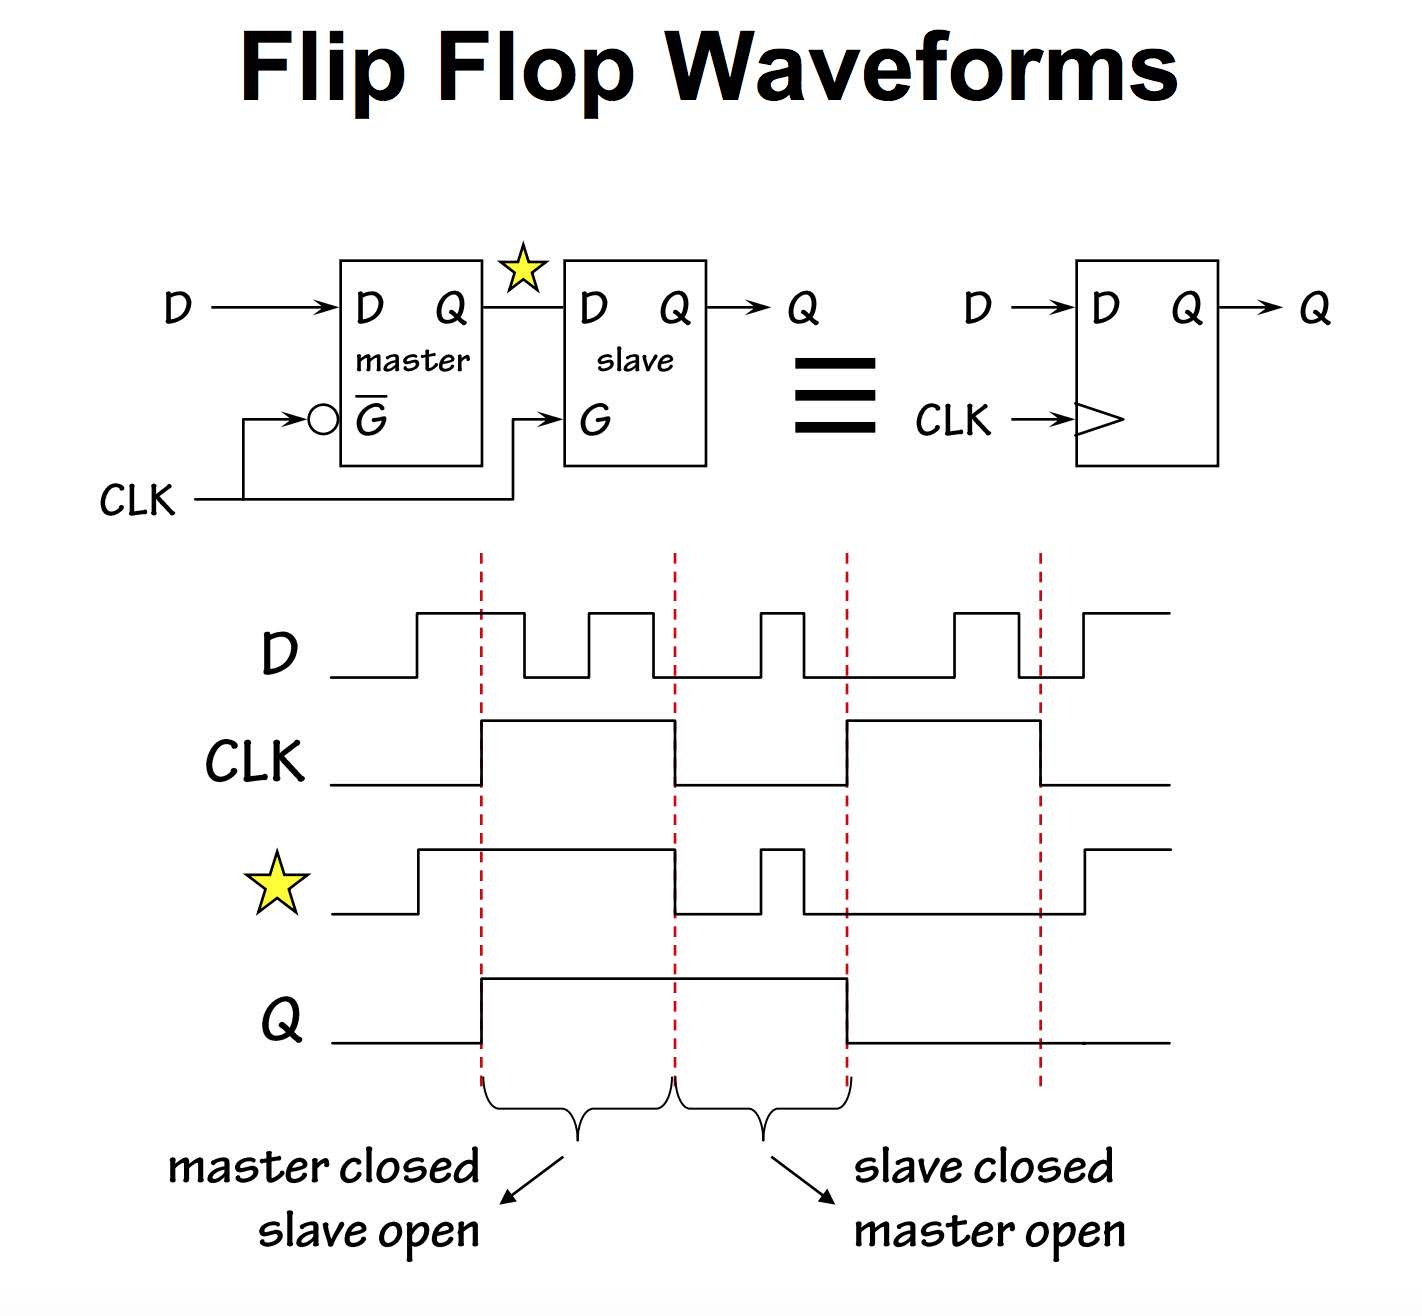
\includegraphics[width = 4.5cm]{Flip_flop_waveform}
Note that output wire Q only changes when CLK rises from 0 to 1
\subsubsection{Timing Constraint}
\begin{enumerate}
\item $t_{CD}$ of a D-latch is the time taken for invalid CLK input to produce an invalid output on wire G
\item $T_{PD}$ of a D-latch is the time taken for valid CLK input to produce a valid output on wire G
\end{enumerate}

Sequential Logic Timing Constraint
$t_{1} = t_{CD,R1} + t_{CD,1} > t_{HOLD,R2}$
$t_{2} = t_{PD,R1} + t_{PD,1} < t_{CLK} - t_{SETUP,R2}$


\section{Metastable State}
Properties
\begin{enumerate}
\item It corresponds to an invalid logic level
\item Unstable equilibrium which will settle to valid 0 or 1 eventually
\item Settling can be arbitraily long
\item All bistable system exhibits at least 1 metastable state
\item Cannot be avoided but can be minimize
\end{enumerate}

\subsubsection{Clock Skew}
$t_{1} = t_{CD,R1} + t_{CD,R1} > t_{HOLD,R2} + t_{skew}$ \\
$t_{2} = t_{PD,R1} + t_{PD,CL1} < t_{CLK} - t_{SETUP,R2} + t_{skew}$ \\

Insert FSM







\section{Week 4 material}

\section{Programmable Machines}
\subsection{Programmable control system}
\begin{enumerate}
\item Control processing at each step with FSM
\item Allow different control sequences to be loaded into control FSM
\item Re-use data path and reconfigure FSM to compute new function
\end{enumerate}
\subsection{Short-comings}
\begin{enumerate}
\item Tiny repertoire of operation
\item Unable to generate and execute a new program
\item Limited storage
\end{enumerate}
\subsection{Finate State Machine: Enumeration}
FSM with \textit{i} inputs, \textit{o} outputs, \textit{s} states 
\begin{enumerate}
\item Truth table has $2^{i + s}$ rows with (o + s) columns each
\item $2^{(o + s) 2^{i + s}}$ max state
\item Limitation : cannot solve problems with arbitrarily many states
\end{enumerate}

\subsection{Turing Machines}
Turing Machine Specification
\begin{enumerate}
\item Doubly-infinite tape
\item Discrete symbol positions
\item Finite alphabet
\item Control FSM \\
Inputs - Current Symbol \\
Outputs - Write 0/1 , move Left/Right 
\item Initial Starting State {S0}
\item Halt State{Halt}
\end{enumerate}
Properties
\begin{enumerate}
\item Can be used to compute integer functions of form $y = T_{k}[x]$ 
\item Where k: FSM index, x: input tape configuration, y: output tape configuration. \\
*Not all integer functions can be computed with Turing Machines
\item Computable functions : f(x) computable $\Leftrightarrow \exists k : \forall x: f(x) = T_{k}[x] = f_{k}(x)$
\item Church-Turing Hypothesis states that any computable function is computable by a TM
\end{enumerate}

\subsection{Universal Functions and Universality}
Universal function: $U(k,j) = T_{k}(j)$ \\
U is comptable by a Turing Machine \\
$\rightarrow$ k encodes a 'program' \\
$\rightarrow$ j encodes the input data to be used \\
$\rightarrow T_{u}$ interprets program





\end{multicols*}

\begin{multicols*}{4}
\setlength{\premulticols}{1pt}
\setlength{\postmulticols}{1pt}
\setlength{\multicolsep}{1pt}
\setlength{\columnsep}{2pt}

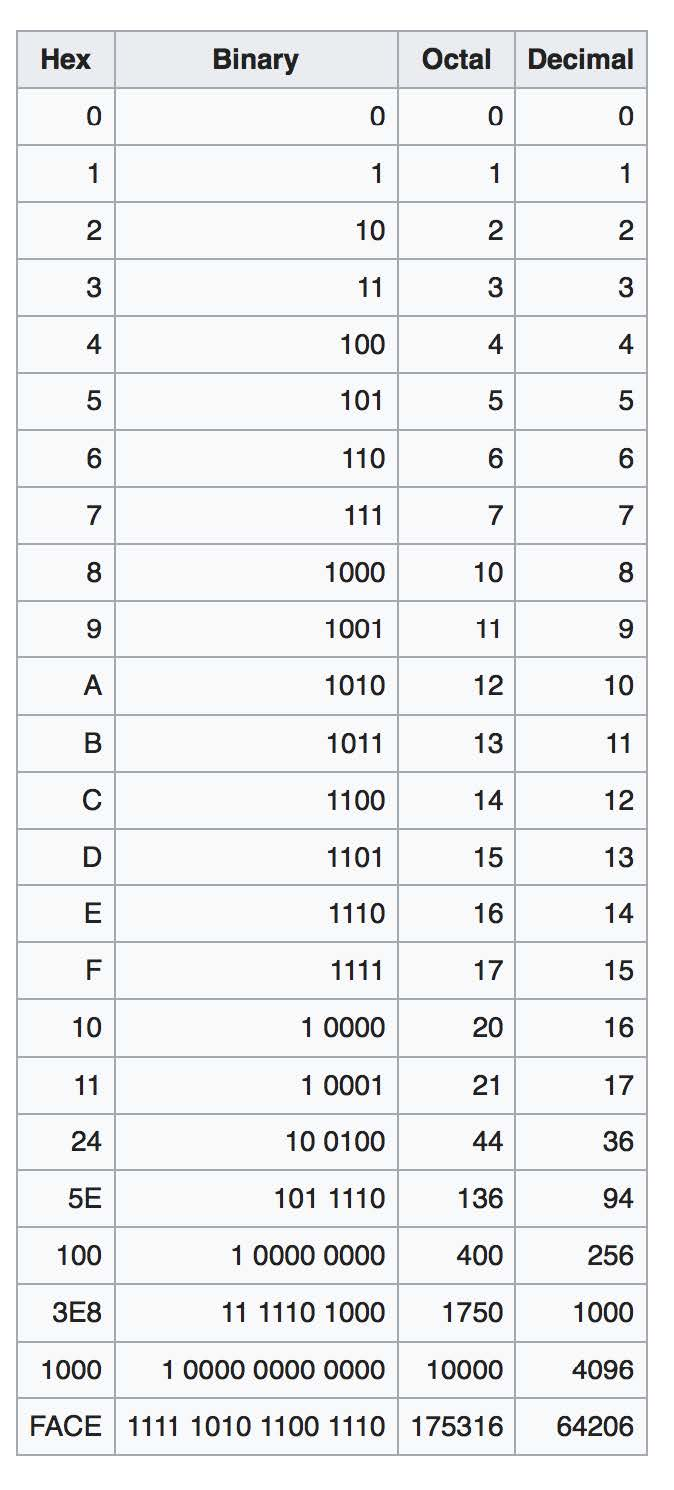
\includegraphics[width = 7cm]{Conversion_table}
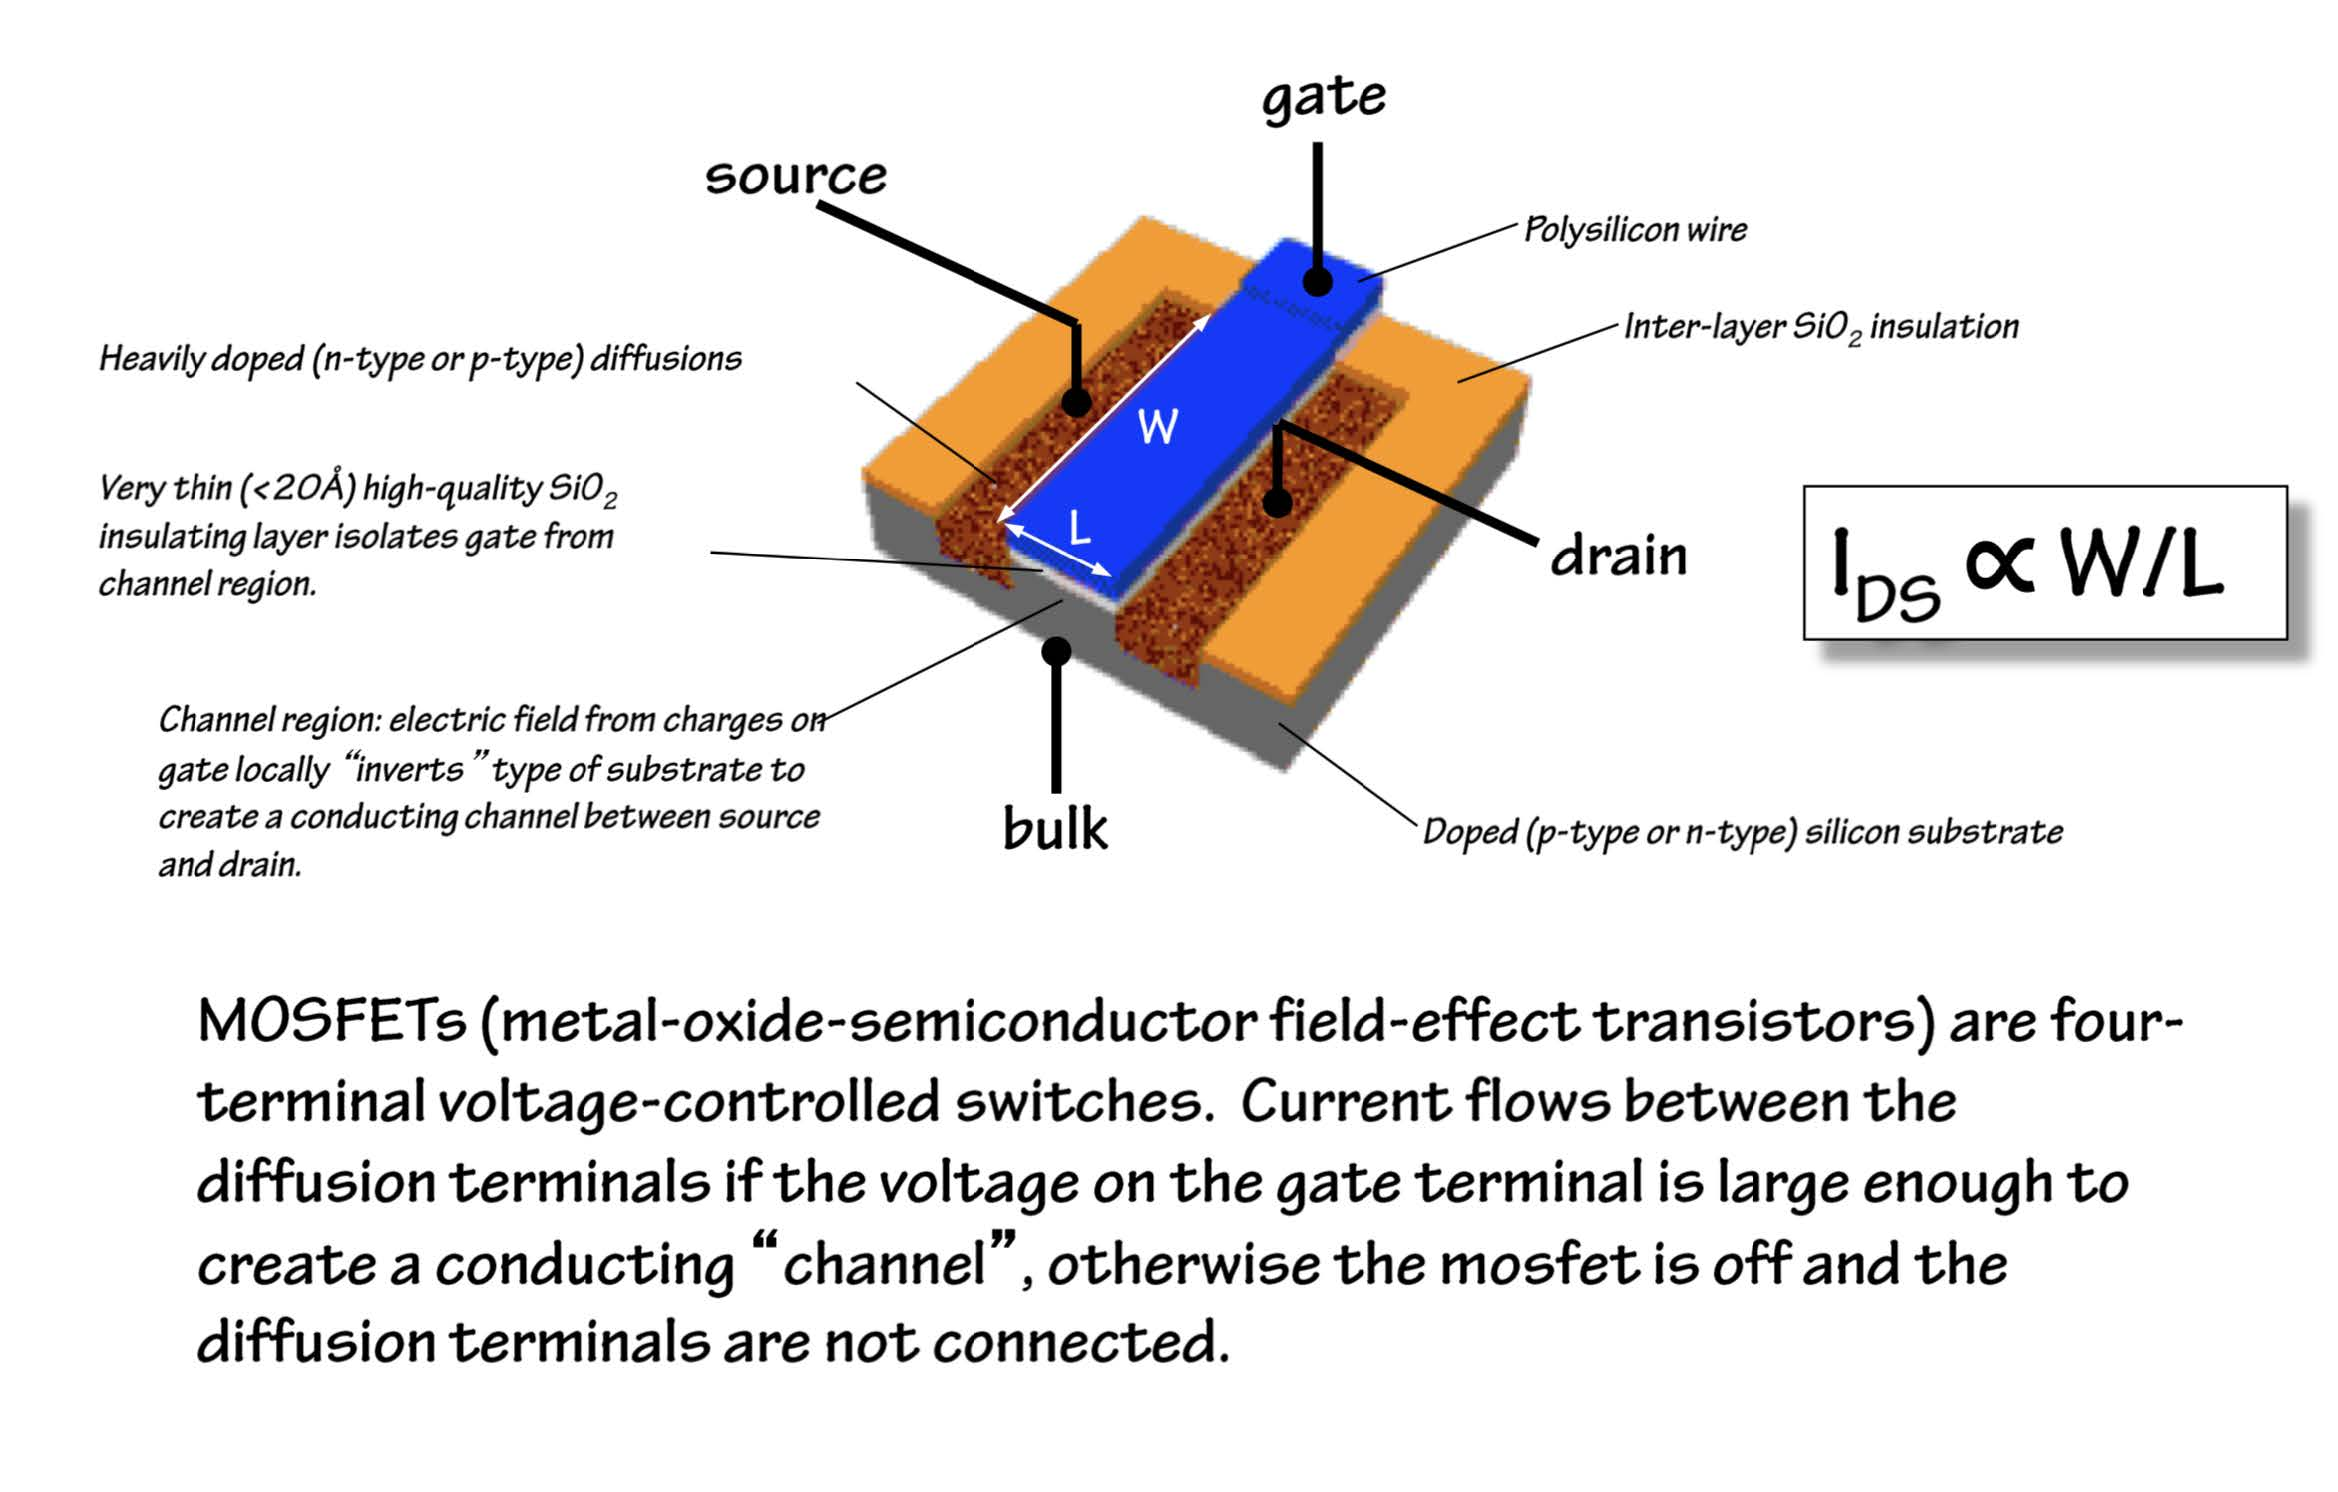
\includegraphics[width = 7cm]{Mosfet}
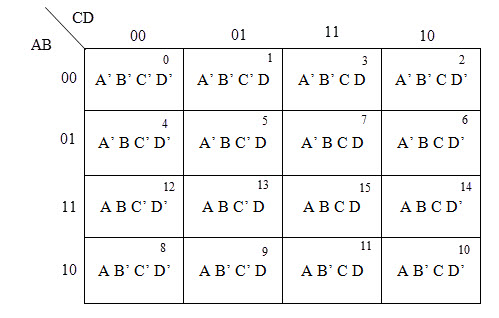
\includegraphics[width = 7cm]{K-map}
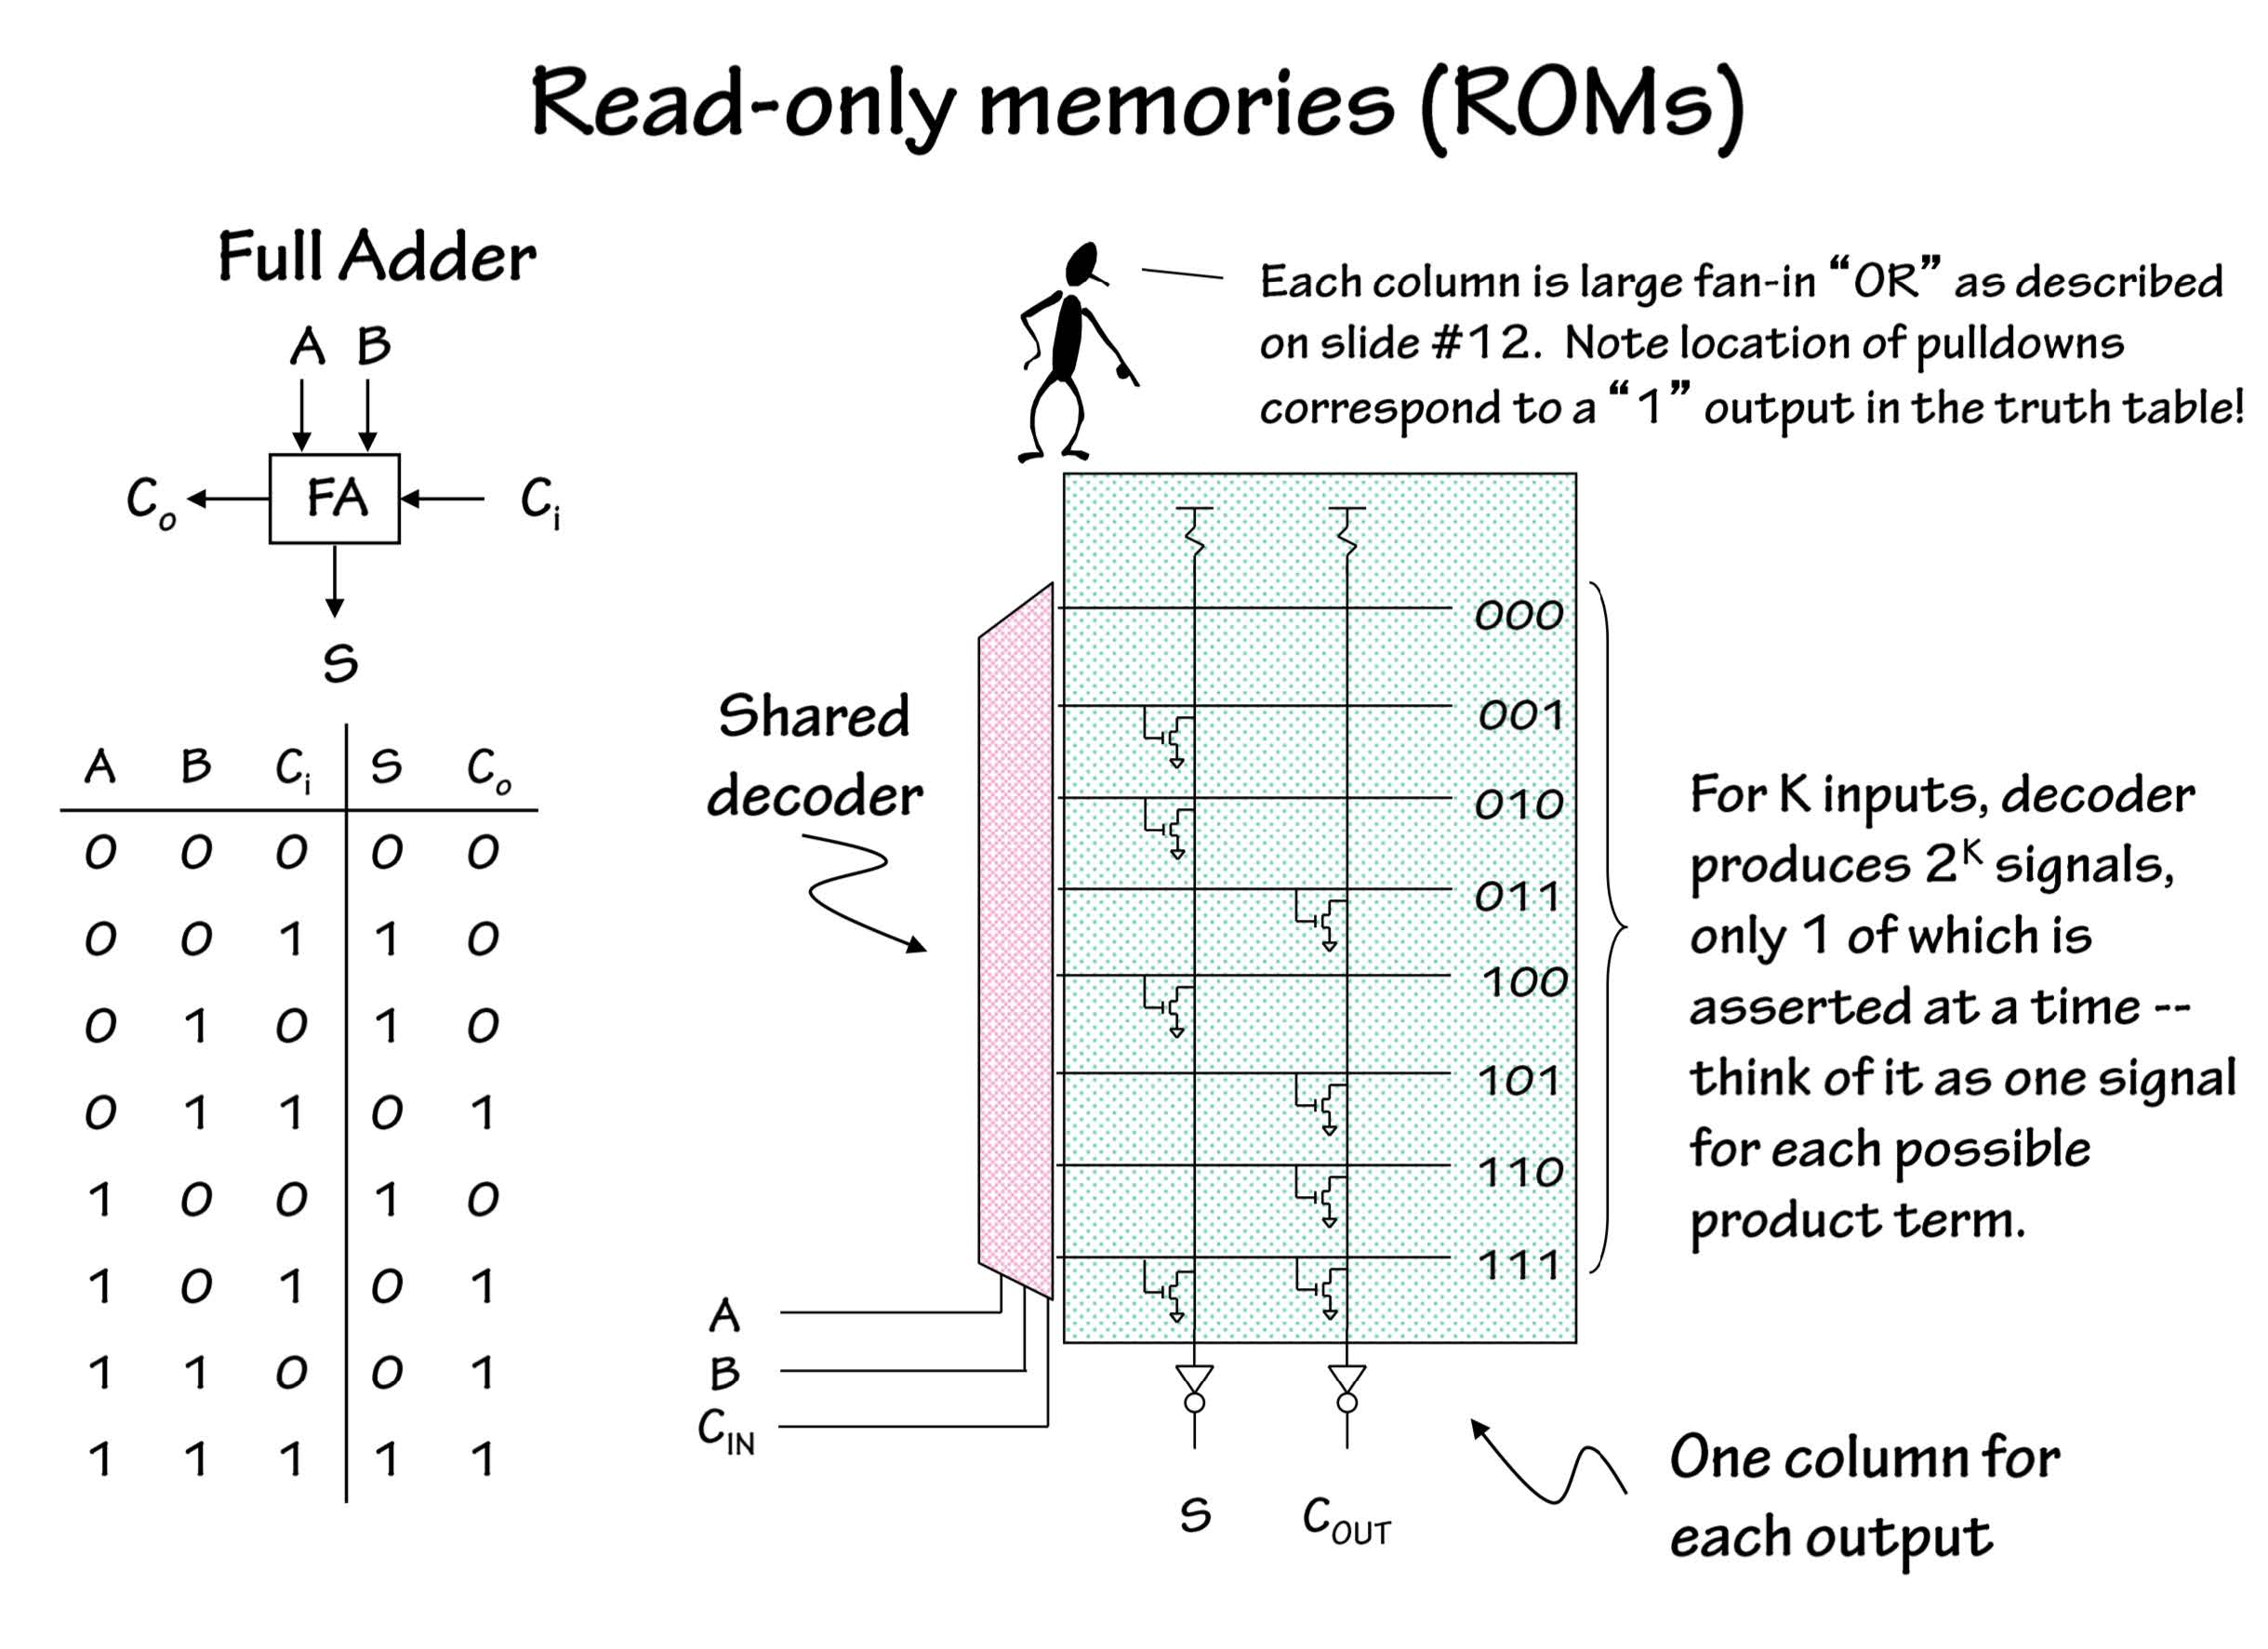
\includegraphics[width = 7cm]{ROM}
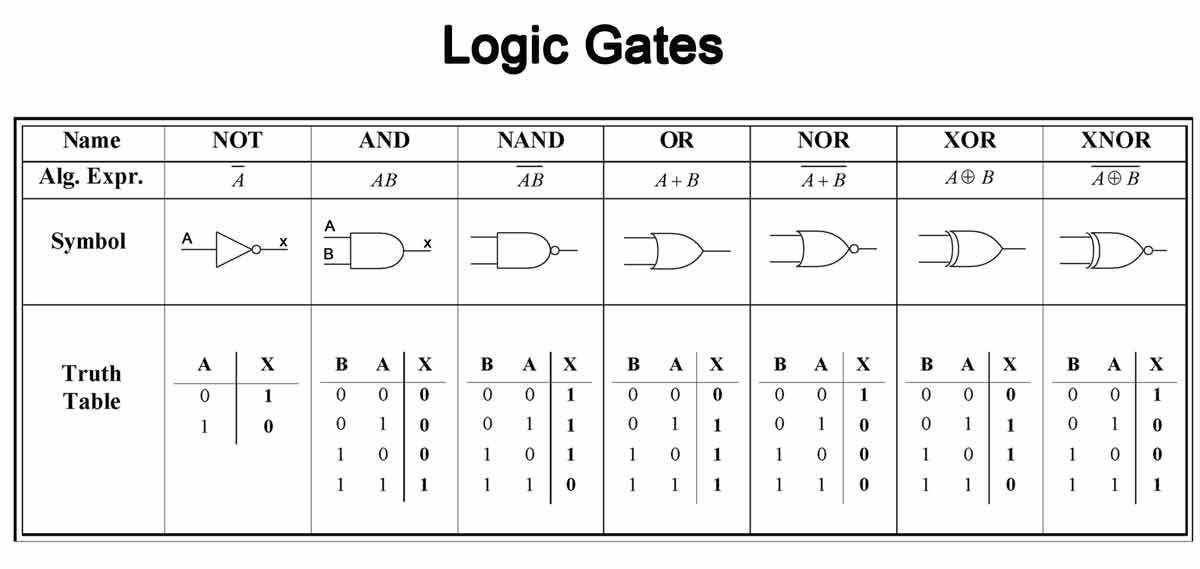
\includegraphics[width = 7cm]{Logic_gates}
\end{multicols*}
\end{document}